\documentclass[twoside,numberorder]{csbachelor}

%==============================================================
%==============================================================

\usepackage{url}
\usepackage{subfigure}

% 张海:其他引用
\usepackage[hidelinks]{hyperref}
\usepackage{pdfpages}

% 一些全局工具的定义
\DeclareMathOperator*{\argmin}{arg\,min}
\DeclareMathOperator*{\argmax}{arg\,max}

%==============================================================
%==============================================================

\begin{document}

\pagestyle{empty}

%==============================================================
%==============================================================

  % 论文题目:{中文}{英文}
  \zjutitle{标题}
           {Title}
  % 作者:{中文姓名}{英文}{学号}
  \zjuauthor{姓名}{Name}{313XXXXXXXX}
  % 指导教师:{导师中文名}{导师英文名}
  \zjumentor{导师姓名}{Supervisor name}
  % 个人信息:{年级}{专业名称}
  \zjuinfo{2013级}{计算机科学与技术}
  % 学院信息:{学院中文}{学院英文}
  \zjucollege{计算机科学与技术学院}{College of Computer Science and Technology}
  % 日期:{Submitted Date}
  %\zjudate{2017-03-29}

%==============================================================

  %%============================================================
%% 中文封面

\thispagestyle{empty}

\vspace{5mm}

\begin{center}
  
\includegraphics[width=108mm]{images/zjdx}
\end{center}

\vspace{10mm}

{
\heiti\erhao\bfseries
\centerline{本~~科~~生~~毕~~业~~设~~计}
\centerline{开题报告}
\vspace{18mm}
}

\begin{center}
  
\includegraphics[width=32mm]{images/standxb}
\end{center}

\vspace{15mm}

{
\songti\sanhao\bfseries
\begin{tabbing}
  \hspace{20mm}
  \= 学生姓名:\= \underline{\makebox[7cm]{\zjuauthornamec}} \\[2mm]
  \> 学生学号: \> \underline{\makebox[7cm]{\zjuauthorid}} \\[2mm]
  \> 指导教师: \> \underline{\makebox[7cm]{\zjumentorc}} \\[2mm]
  \> 年级专业: \> \underline{\makebox[7cm]{\zjugrade\zjumajor}} \\[2mm]
  \> 所在学院: \> \underline{\makebox[7cm]{\zjucollegec}} \\[2mm]
\end{tabbing}
}

%%============================================================
% empty page for two-page print
\ifthenelse{\equal{\zjuside}{T}}{%
  \newpage\mbox{}%
  \thispagestyle{empty}}{}


  \newpage

\thispagestyle{empty}

{
\setlength{\parindent}{0em}
\renewcommand{\baselinestretch}{2}
\songti\sihao\bfseries

一、 \; 题目: \; \underline{\makebox[24em]{\zjutitlec}}

\vspace{2em}

二、 \; 指导教师对开题报告、外文翻译和中期报告的具体要求:

1. \; 开题报告要求: \; 要求。

2. \; 外文翻译要求: \; 要求。

3. \; 中期报告要求: \; 要求。

\vspace{8cm}
}

{
\songti\xiaosi\bfseries
\begin{flushright}
  指导教师(签名) \; \underline{\hspace{6em}} \\
  年 \qquad 月 \qquad 日
\end{flushright}
}

\ifthenelse{\equal{\zjuside}{T}}{\newpage\mbox{}\thispagestyle{empty}}{}


  \thispagestyle{empty}

{
  \setlength{\parindent}{0em}
  \renewcommand{\baselinestretch}{2}

  {
    \stfangsong\sanhao\bfseries
    \centering
    毕业设计开题报告、外文翻译的考核 \par
  }

  {
    \songti\sihao\bfseries
    导师对开题报告、外文翻译的评语及成绩评定:

    \vspace{10em}

    {
      \renewcommand{\baselinestretch}{1}

      \begin{flushright}

        \begin{tabular}{|c|c|c|c|}
          \hline
          成绩比例 & \parbox[c]{3.6em}{\xiaosi 开题报告 \\ 占(20\%) \vspace{0.25em}} & \parbox[c]{3.6em}{\xiaosi 外文翻译 \\ 占(10\%) \vspace{0.25em}} \\
          \hline
          分值 & & \\
          \hline
        \end{tabular}

        \vspace{2em}

        {
          \songti\xiaosi\bfseries
          导师签名 \; \underline{\hspace{6em}} \\
          年 \qquad 月 \qquad 日 \par
        }
      \end{flushright}
    }
  }

  \vspace{2em}

  {
    \songti\sihao\bfseries
    学院盲审专家对开题报告、外文翻译的评语及成绩评定:

    \vspace{10em}

    {
      \renewcommand{\baselinestretch}{1}

      \begin{flushright}

        \begin{tabular}{|c|c|c|c|}
          \hline
          成绩比例 & \parbox[c]{3.6em}{\xiaosi 开题报告 \\ 占(20\%) \vspace{0.25em}} & \parbox[c]{3.6em}{\xiaosi 外文翻译 \\ 占(10\%) \vspace{0.25em}} \\
          \hline
          分值 & & \\
          \hline
        \end{tabular}

        \vspace{2em}

        {
          \songti\xiaosi\bfseries
          开题报告审核负责人(签名/签章) \; \underline{\hspace{6em}} \par
        }
      \end{flushright}
    }
  }

  \newpage

  {
    \stfangsong\sanhao\bfseries
    \centering
    毕业设计中期报告考核 \par
  }

  {
    \songti\sihao\bfseries
    导师对中期报告的评语及成绩评定:

    \vspace{10em}

    {
      \renewcommand{\baselinestretch}{1}

      \begin{flushright}

        \begin{tabular}{|c|c|c|c|}
          \hline
          成绩比例 & \parbox[c]{3.6em}{\xiaosi 中期报告 \\ 占(10\%) \vspace{0.25em}} \\
          \hline
          分值 & \\
          \hline
        \end{tabular}

        \vspace{2em}

        {
          \songti\xiaosi\bfseries
          导师签名 \; \underline{\hspace{6em}} \\
          年 \qquad 月 \qquad 日 \par
        }
      \end{flushright}
    }
  }
}


  \tableofcontents
  \thispagestyle{toc}
  %\chaptermark{目录}

  \mainmatter

  {
    \pagestyle{kaitibaogao}
    \makeatletter
      \let\ps@plain\ps@kaitibaogao
    \makeatother
    \chapter*{``\zjutitlec'' 开题报告}

\section{项目背景}

\cite{article1}

\section{目标和任务}

\section{可行性分析}

\section{初步技术方案和关键技术考虑}

\section{预期工作结果}

\section{进度计划}

本项目的整体计划如下表所示:

\begin{table}[!htbp]
\centering
\begin{tabular}{|l|l|}
\hline
时间 & 主要工作 \\ \hline
2017年1月 & 开始 \\ \hline
\end{tabular}
\caption{项目进度计划}
\label{table:schedule}
\end{table}

\bibliographystyle{data/gbt7714-2005}
{
\renewcommand{\chapter}[2]{\section*{#2}\addcontentsline{toc}{section}{#2}}
\bibliography{data/kaitibaogao}
}

% 按文章长度需要启用
\ifthenelse{\equal{\zjuside}{T}}{\newpage\mbox{}\thispagestyle{empty}}{}

  }

  {
    \pagestyle{waiwenfanyi}
    \makeatletter
      \let\ps@plain\ps@waiwenfanyi
    \makeatother
    \setcounter{page}{1}

    \renewcommand{\addcontentsline}[3]{}

    {
\renewcommand{\baselinestretch}{1.25}\selectfont

{
  \titleformat{\chapter}[block]{\erhao\songti\bfseries\filcenter}{}{0em}{}{}
  \chapter{本科毕业设计外文翻译}
}

{
  \setlength{\parindent}{0em}

  文献原文:

  A. Bravo, C. Delta. How to translate a sample paper. 2017. \par
}

\vspace{2em}

{
  \renewcommand{\cleardoublepage}{}
  \renewcommand{\clearpage}{}
  \titleformat{\chapter}[block]{\sanhao\songti\bfseries\filcenter}{}{0em}{}{}
  \chapter*{外文翻译标题}
}

\section*{摘要}

\section{前言}

\begin{figure}[!htbp]
\centering

\includegraphics[width=\linewidth,keepaspectratio]{data/waiwenfanyi/placeholder.png}
\caption{Placeholder}
\label{figure:placeholder}
\end{figure}

图~\ref{figure:placeholder}

手动引用~1 {[}1{]}

\section{参考文献}

\begin{itemize}
\item [{[}1{]}] A. Baker, C. Dog. How to make a sample reference. 1938.
\end{itemize}
}

% 按文章长度需要启用
%\ifthenelse{\equal{\zjuside}{T}}{\newpage\mbox{}\thispagestyle{empty}}{}

  }

  \backmatter

  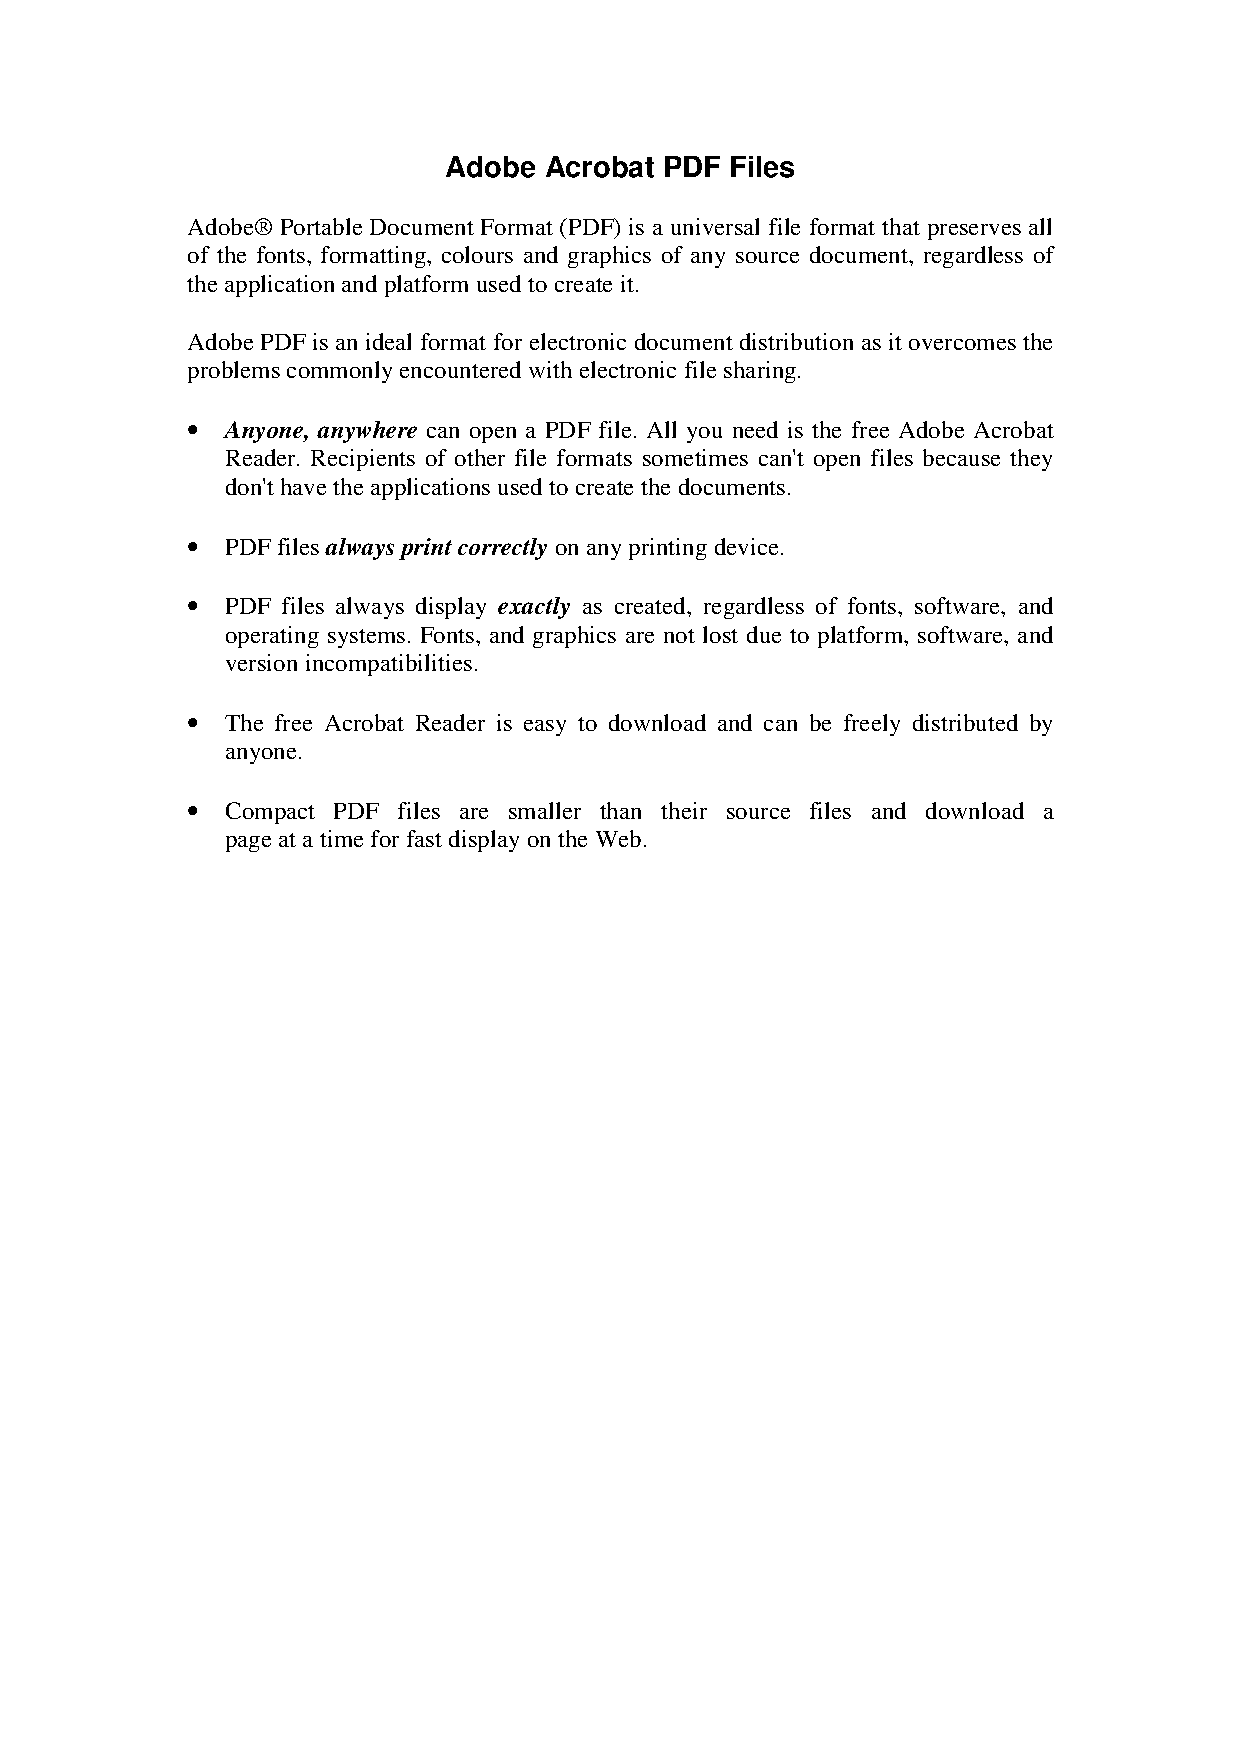
\includepdf[pages=-]{data/waiwenyuanwen.pdf}

\end{document}
